\noindent Considérons toujours un \texttt{MDP} avec :
\begin{itemize}[label=\textbullet]
    \item des états $s\in S$
    \item des actions $a\in A$
    \item un modèle $T(s,a,s')$
    \item une fonction de récompense $R(s,a,s')$
\end{itemize}
Nous sommes toujours à la recherche d'une politique $\pi(s)$. Cependant, nous ne connaissons plus pour autant le modèle ni la
fonction de récompense. Le but est d'apprendre quelles actions prendre dans quel état pour maximiser la récompense. Un schéma
qu'il faut avoir en tête est le suivant :
\begin{figure}[H]
    \centering
    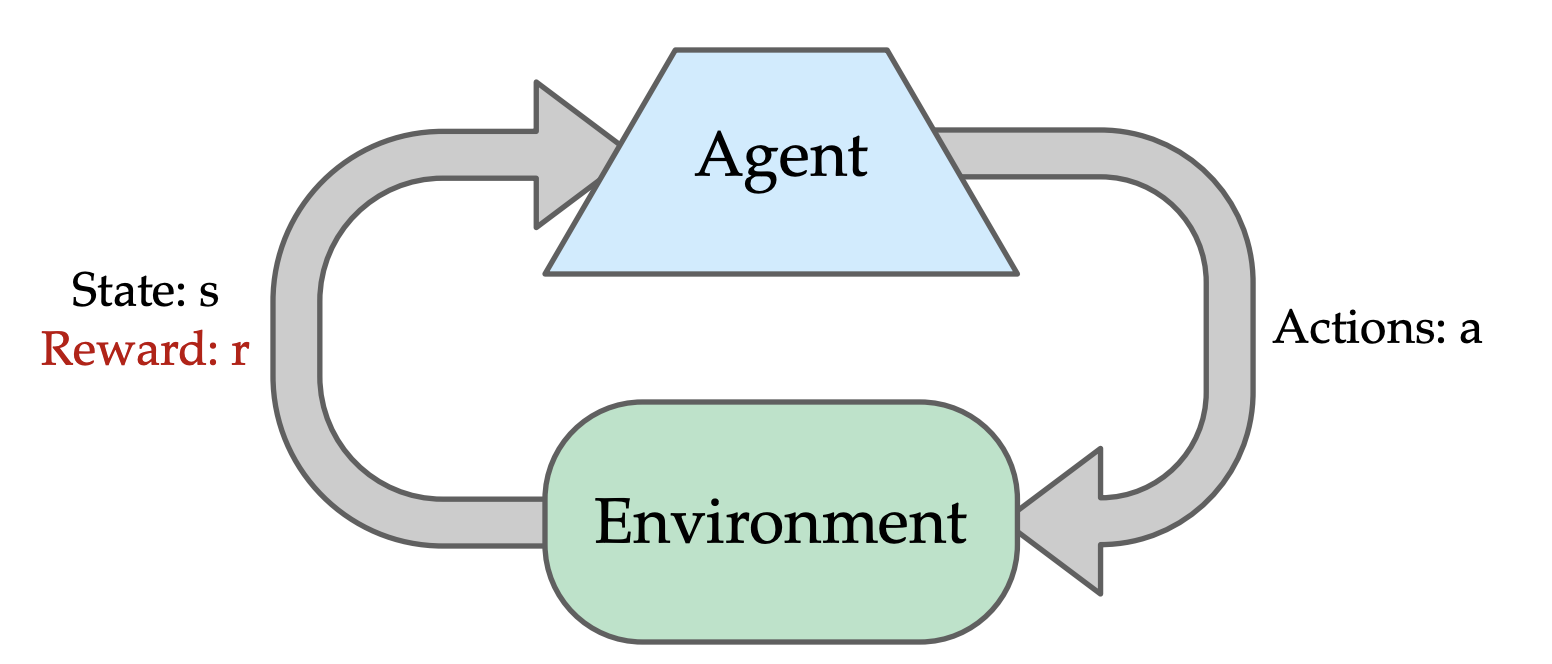
\includegraphics[width=0.5\linewidth]{pictures/rl_scheme.png}
    \caption{Schéma de l'apprentissage par renforcement}
    \label{fig:rl_scheme}
\end{figure}
\noindent L'idée est la suivante :
\begin{itemize}[label=\textbullet]
    \item On reçoit un feedback de l'environnement (reward).
    \item L'utilité de l'agent est définie par la fonction de récompense.
    \item L'agent doit apprendre à maximiser les récompenses attendues.
    \item Tous l'apprentissage est basé sur des observations d'output de l'environnement.
\end{itemize}

\subsection{Passive Reinforcement Learning} % (fold)
\subsubsection{Model-based Passive RL} % (fold)
\label{ssub:model_based_passive_rl}
\begin{definition}{Model-based Passive RL}{}
    Le but est d'apprendre le modèle MDP depuis les expériences et ensuite de résoudre le MDP appris.
\end{definition}
Le model-based RL est donc divisé en deux étapes :
\begin{enumerate}
    \item Apprendre le modèle MDP empirique 
    \begin{enumerate}
        \item Compter les résultats $s'$ pour chaque transition $(s,a)$.
        \item Normaliser afin de donner une estimation $\hat{T}(s,a,s')$.
        \item Découvrir chaque $\hat{R}(s,a,s')$ quand on fait $(s,a,s')$.
    \end{enumerate}
    \item Résoudre le MDP appris, en utilisant par exemple la value iteration.
\end{enumerate}

\subsubsection{Model-free Passive RL} % (fold)
\label{ssub:model_free_passive_rl}
\begin{definition}{Model-free Passive RL}{}
    Renoncer à l'apprentissage du modèle MDP et apprendre directement la fonction de valeur $V$ ou $Q$.\\
    \begin{itemize}[label=\textbullet]
        \item $V$ fait référence à value learning où on apprend la valeur d'une politique fixe. Elle est constituée
        de deux approches : l'\textbf{évalutation directe}(cf.\ref{ssubsub:direct_evaluation}) et le \textbf{TD learning}
        (cf.\ref{ssubsub:td_learning}).
        \item $Q$ fait référence à Q-learning où on apprend les Q-valeurs de la politique optimale. L'approche utilisée
        est une Q-version du TD learning.
    \end{itemize}
\end{definition}
Autrement dit, il faut évaluer une politique. On a en entrée un politique fixe $\pi(s)$ et on ne connait ni les transitions
ni les récompenses. Le but est d'apprendre la valeur des états.\\
Dans notre cas on a :
\begin{itemize}[label=\textbullet]
    \item L'apprenant est "dans le coup"
    \item Pas le choix des actions prises
    \item Il suffit d'exécuter la politique et d'apprendre des expériences
    \item Ce n'est pas \texttt{OFFLINE} car l'apprenant prend des actions dans le monde.
\end{itemize}

\subsubsubsection{Direct evaluation} % (fold)
\label{ssubsub:direct_evaluation}
Le \textbf{but} est de calculer les valeurs pour chaque état sous la politique $\pi$. L'\textbf{idée} est de faire la moyenne
de l'ensemble des valeurs observées de l'échantillon, pour ce faire :
\begin{itemize}[label=\textbullet]
    \item On agit par rapport à la politique $\pi$.
    \item A chaque fois qu'on visite un état, on met à jour la somme des récompenses.
    \item On fait la moyenne de ces échantillons.
\end{itemize}
Les avantages et les défauts de cette méthode sont les suivants :
\begin{itemize}[label=\textbullet]
    \item[$+$] Simple
    \item[$+$] On a pas besoin de connaitre ni T ni R.
    \item[$+$] Il finitpar calculer les valeurs moyennes correctes en utilisant uniquement les transitions de l'échantillon.
    \item[$-$] Il y a une perte d'information entre les connexions entre les états.
    \item[$-$] Chaque état doit être apppris indépendamment.
    \item[$-$] Il faut beaucoup de temps pour apprendre. 
\end{itemize}

\subsubsubsection{TD learning} % (fold)
\label{ssubsub:td_learning}
Une question qui se pose est : Pourquoi ne pas utiliser la Poilicy Evaluation?\\
Sur l'équation de Bellman suivante : (pour $V_0^{\pi}(s)=0$)
\begin{equation*}
    V_{k+1}^{\pi}(s)=\sum_{s'}T(s,\pi(s),s')[R(s,\pi(s),s')+\gamma V_k^{\pi}(s')]
\end{equation*}
À chaque tour, on remplace V avec un V une étape plus loin. Cette approche exploite pleinement les connexions entre les états.
Malheuresement, il faut connaitre T et R. La question est maintenant : Comment pouvons nous mettre à jour la valeur de V sans
connaître T et R?

L'\textbf{idée} est d'apprendre de chaque expérience au fur et à mesure, il faut donc mettre à jour $V(s)$ à chaque fois qu'on
expérimente une transition $(s,a,s',r)$. Les résultats probables $s'$ contribueront à des mises à jour plus fréquentes. Dès lors,
il y a une différence temporelle (Temporal Difference Value Learning) entre les valeurs de $V(s)$ et $V(s')$, quand on déplace 
les valeurs vers la valeur du successeur quel qu'il soit, on fait une moyenne dynamique. On a :
\begin{itemize}[label=\textbullet]
    \item Sample of $V(s)$: $\text{sample}=R(s,\pi(s),s')+\gamma V^\pi(s')$
    \item Update to $V(s)$: $V(s)\leftarrow (1-\alpha)V^\pi(s)+\alpha\text{ sample}$
    \item La même mise à jour : $V(s)\leftarrow V^\pi(s)+\alpha(\text{sample}-V^\pi(s))$
\end{itemize}
Le fait de faire une mise à jour de l'interpolation en cours ($\bar{x}_n=(1-\alpha)\cdot\bar{x}_{n-1}+\alpha\cdot x_n$) permet
de rendre les états récents plus importants tandis que les états plus anciens sont moins importants. Si le taux d'apprentissage
$\alpha$ diminue, les moyennes convergent.\\
Le \textbf{problème} avec le TD learning est que c'est un moyen sans modèle d'évaluer les politiques en imitant les mises à jour
de Bellman avec des moyennes d'échantillons en cours d'exécution. SI on veut transformer les valeurs en une nouvelle politique,
on est perdus, effectivement :
\begin{equation*}
    \begin{aligned}
        \pi(s)&=\max\limits_{a} Q(s,a)\\
        Q(s,a)&=\sum_{s'}T(s,a,s')[R(s,a,s')+\gamma V(s')]
    \end{aligned}
\end{equation*}

\subsubsubsection{Q-learning} % (fold)
\label{ssubsub:q_learning}
Value iteration trouve des valeurs successives (limitées par une profondeur max) mais les $Q-values$ sont plus pratiques, 
elles fonctionnent ainsi :
\begin{itemize}[label=\textbullet]
    \item On commence avec $Q_0(s,a)=0$.
    \item Pour un $Q_k$ donné, on calcule $Q_{k+1}$ pour tous les q-états :
    \begin{equation*}
        Q_{k+1}(s,a)\leftarrow\sum_{s'}T(s,a,s')[R(s,a,s')+\gamma\max\limits_{a'}Q_k(s',a')]
    \end{equation*}
\end{itemize}
A partir d'un échantillon $(s,a,s',r)$, on peut mettre à jour $Q(s,a)$ :
\begin{equation*}
    \text{sample} = R(s,a,s')+\gamma\max\limits_{a'}Q(s',a')
\end{equation*}
On voit qu'on a plus d'évaluation de politique. On peut intégrer la nouvelle estimation dans la moyenne dynamique :
\begin{equation*}
    Q(s,a)\leftarrow (1-\alpha)Q(s,a)+\alpha\text{ sample}
\end{equation*}
Voici les propriétés de Q-learning :
\begin{itemize}[label=\textbullet]
    \item Q-learning converge vers les Q-valeurs optimales même si on agit de manière suboptimale.
    \item C'est une méthode d'apprentissage "off-policy"
\end{itemize}
Cependant, il faut faire attention à:
\begin{itemize}[label=\textbullet]
    \item Parcourir suffisament longtemps.
    \item Il faut parfois donner une valeur très petite à $\alpha$ mais il ne faut pas le diminuer trop rapidement.
    \item Il n'y a pas vraiment d'importance à la façon dont on choisit les actions.
\end{itemize}